\documentclass[notes,11pt, aspectratio=169]{beamer}

\usepackage{pgfpages}
% These slides also contain speaker notes. You can print just the slides,
% just the notes, or both, depending on the setting below. Comment out the want
% you want.
\setbeameroption{hide notes} % Only slide
%\setbeameroption{show only notes} % Only notes
%\setbeameroption{show notes on second screen=right} % Both

%\usepackage{helvet}
%\usepackage[default]{lato}
\usepackage{bookman}
\usepackage{array}


\usepackage{tikz}
\usepackage{verbatim}
\setbeamertemplate{note page}{\pagecolor{yellow!5}\insertnote}
\usetikzlibrary{positioning}
\usetikzlibrary{snakes}
\usetikzlibrary{calc}
\usetikzlibrary{arrows}
\usetikzlibrary{decorations}
%\usetikzlibrary{decorations.markings}
%\usetikzlibrary{shapes.misc}
\usetikzlibrary{matrix,shapes,arrows,fit, arrows.meta, tikzmark}
\tikzset{
	-Latex,auto,node distance =1 cm and 1 cm,semithick,
	state/.style ={ellipse, draw, minimum width = 0.7 cm},
	point/.style = {circle, draw, inner sep=0.04cm,fill,node contents={}},
	bidirected/.style={Latex-Latex,dashed},
	el/.style = {inner sep=2pt, align=left, sloped}
}
\usepackage{amsmath}
\usepackage{mathpazo}
\usepackage{hyperref}
\usepackage{lipsum}
\usepackage{multimedia}
\usepackage{graphicx}
\usepackage{multirow}
\usepackage{graphicx}
\usepackage{dcolumn}
\usepackage{bbm}
\newcolumntype{d}[0]{D{.}{.}{5}}
\usepackage{makecell}

% Tabular line breaks
\renewcommand\theadalign{bc}
\renewcommand\theadfont{\bfseries}
\renewcommand\theadgape{\Gape[4pt]}
\renewcommand\cellgape{\Gape[4pt]}


\usepackage{changepage}
\usepackage{appendixnumberbeamer}
\newcommand{\beginbackup}{
   \newcounter{framenumbervorappendix}
   \setcounter{framenumbervorappendix}{\value{framenumber}}
   \setbeamertemplate{footline}
   {
     \leavevmode%
     \hline
     box{%
       \begin{beamercolorbox}[wd=\paperwidth,ht=2.25ex,dp=1ex,right]{footlinecolor}%
%         \insertframenumber  \hspace*{2ex} 
       \end{beamercolorbox}}%
     \vskip0pt%
   }
 }
\newcommand{\backupend}{
   \addtocounter{framenumbervorappendix}{-\value{framenumber}}
   \addtocounter{framenumber}{\value{framenumbervorappendix}} 
}

% Math commands
\newcommand{\vect}[1]{\boldsymbol{#1}}


% If you keep your figures in a separate directory, set the path
% to that directory here
\usepackage{graphicx}
\graphicspath{{figures/}}
\usepackage[space]{grffile}
\usepackage{booktabs}

% These are my colors -- there are many like them, but these ones are mine.
\definecolor{cream}{HTML}{E1DAAE}
\definecolor{orange}{HTML}{FF934F}
\definecolor{red}{HTML}{CC2D35}
\definecolor{blue}{HTML}{058ED9}
\definecolor{grey}{HTML}{848FA2}
\definecolor{midnight}{HTML}{2D3142}

\hypersetup{
  colorlinks=false,
  linkbordercolor = {white},
  linkcolor = {blue}
}


%% I use a creamy off white for my background
\definecolor{LightBackground}{RGB}{255,253,218}

%% Uncomment this if you want to change the background color to something else
%\setbeamercolor{background canvas}{bg=LightBackground}

%% Change the bg color to adjust your transition slide background color!
\newenvironment{transitionframe}{
  \setbeamercolor{background canvas}{bg=midnight}
  \begin{frame}}{
    \end{frame}
}

%% Remember to change these if you use the DarkBackground
\setbeamercolor{frametitle}{fg=red}
\setbeamercolor{title}{fg=black}
\setbeamertemplate{footline}[frame number]
\setbeamertemplate{navigation symbols}{} 
\setbeamertemplate{itemize items}{-}
\setbeamercolor{itemize item}{fg=midnight}
\setbeamercolor{itemize subitem}{fg=midnight}
\setbeamercolor{enumerate item}{fg=midnight}
\setbeamercolor{enumerate subitem}{fg=midhgt}
\setbeamercolor{button}{bg=cream,fg=midnight,}



% If you like road maps, rather than having clutter at the top, have a roadmap show up at the end of each section 
% (and after your introduction)
% Uncomment this is if you want the roadmap!
% \AtBeginSection[]
% {
%    \begin{transitionframe}
%        \frametitle{Roadmap of Talk}
%        \tableofcontents[currentsection]
%    \end{transitionframe}
% }
\setbeamercolor{section in toc}{fg=blue}
\setbeamercolor{subsection in toc}{fg=orange}
\setbeamersize{text margin left=1em,text margin right=1em} 

\newenvironment{wideitemize}{\itemize\addtolength{\itemsep}{10pt}}{\enditemize}

\usepackage{environ}
\NewEnviron{videoframe}[1]{
  \begin{frame}
    \vspace{-8pt}
    \begin{columns}[onlytextwidth, T] % align columns
      \begin{column}{.58\textwidth}
        \begin{minipage}[t][\textheight][t]
          {\dimexpr\textwidth}
          \vspace{8pt}
          \hspace{4pt} {\Large \sc \textcolor{red}{#1}}
          \vspace{8pt}
          
          \BODY
        \end{minipage}
      \end{column}%
      \hfill%
      \begin{column}{.42\textwidth}
        \colorbox{orange!20}{\begin{minipage}[t][1.2\textheight][t]
            {\dimexpr\textwidth}
            Face goes here
          \end{minipage}}
      \end{column}%
    \end{columns}
  \end{frame}
}

% If you reference citations and want a bibliography add the .bib here, alter settings, and
% uncomment the \printbibliography at the end
%\usepackage[backend=biber, natbib, style=numeric-comp, citestyle=authoryear]{biblatex}
%\usepackage{keyval,ifthen}
%\usepackage{csquotes}
%\addbibresource{causal_inference.bib}

%%%%%%%%%%%%%%%%%%%%%%%%%%%%%%%%%%%%
%%%                              %%%
%%% Start of presentation slides %%%
%%%                              %%%
%%%%%%%%%%%%%%%%%%%%%%%%%%%%%%%%%%%%


\title[]{\textcolor{red}{Template for Better Beamer Presentations}}
\author[EAJ]{}
\institute[UMDCP]{\small{\begin{tabular}{c c c}
\multicolumn{3}{c}{Evan A. Jones} \\
\multicolumn{3}{c}{University of Maryland -- College Park}

%Author A &&  Author B  \\
%Somewhere Fancy && Somewhere Fancy \\

%Author C && Author D   \\
%\multicolumn{3}{c}{Somewhere Fancy} \\
\end{tabular}}}

\date{\today}


\begin{document}

%%% TIKZ STUFF
\tikzset{   
        every picture/.style={remember picture,baseline},
        every node/.style={anchor=base,align=center,outer sep=1.5pt},
        every path/.style={thick},
        }
\newcommand\marktopleft[1]{%
    \tikz[overlay,remember picture] 
        \node (marker-#1-a) at (-.3em,.3em) {};%
}
\newcommand\markbottomright[2]{%
    \tikz[overlay,remember picture] 
        \node (marker-#1-b) at (0em,0em) {};%
}
\tikzstyle{every picture}+=[remember picture] 
\tikzstyle{mybox} =[draw=black, very thick, rectangle, inner sep=10pt, inner ysep=20pt]
\tikzstyle{fancytitle} =[draw=black,fill=red, text=white]
%%%% END TIKZ STUFF

% Title Slide
\begin{frame}
\maketitle
  \centering Prepared for [insert venue here].
\end{frame}

% INTRO
\begin{frame}{[Intro Frame]}
\begin{columns}[T] % align columns
\begin{column}{.58\textwidth}
  \begin{wideitemize}
    \item This is a witty comment that makes some in the audience laugh and offends others
    \item This is a less pompous comment that brings the audience back down.
    \item This is a thought-provoking question.
%    \item Read \emph{\textcolor{blue}{\href{https://www.amazon.com/Better-Presentations-Guide-Scholars-Researchers/dp/0231175213/}{Jon Schwabish's ``Better Presentations''}}}
  \end{wideitemize}
\end{column}%
\hfill%
\begin{column}{.38\textwidth}
  \makebox[\linewidth][c]{
    \resizebox{\linewidth}{!}{
      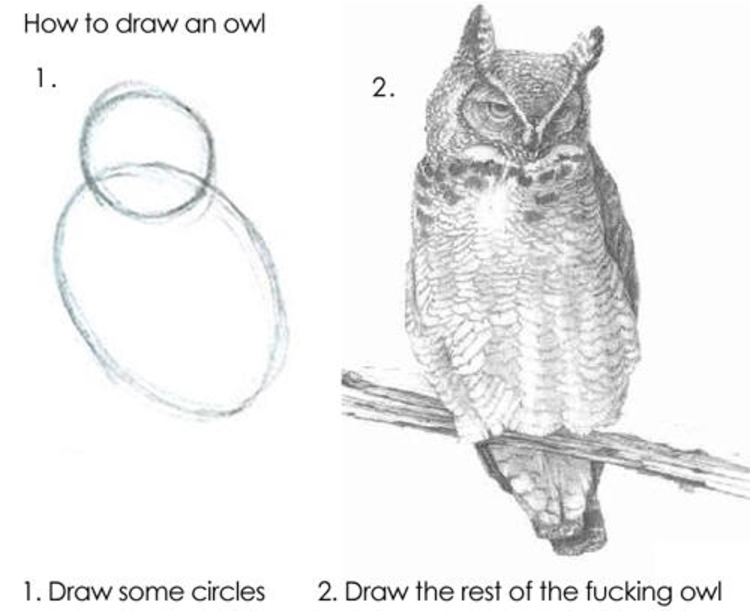
\includegraphics{how-to-draw-an-owl.pdf}
    }
  }
\end{column}%
\end{columns}
\end{frame}

\begin{frame}{Outline}
  \begin{wideitemize}
    \item First topic
    \item Second topic
    \item etc
  \end{wideitemize}
\end{frame}


%% Use this as a fill-in template for transition slides
%\section{}
%\begin{transitionframe}
%  \begin{center}
%    { \Huge \textcolor{blue}{}}
%  \end{center}
%\end{transitionframe}


%\begin{frame}[fragile]{New environments to improve transition and spacing}
%\begin{columns}[T] % align columns
%\begin{column}{.7\textwidth}
%
%  \begin{wideitemize}
%    \item Break up sections using \textcolor{red}{\texttt{transitionframe}} instead of \textcolor{red}{\texttt{frame}}
%      { \scriptsize
%\begin{verbatim}
%\begin{transitionframe}
%  \begin{center}
%    { \Huge \textcolor{}{Spacing and Words}}
%  \end{center}
%\end{transitionframe}
%\end{verbatim}
%}
%    \item  Use my \textcolor{red}{\texttt{wideitemize}} environment instead of \textcolor{red}{\texttt{itemize}}
%      \begin{itemize}
%      \item This environment automatically spaces wide between items
%      \item That way you don't write too much text on a slide!
%      \item Rule of thumb 1: \textcolor{green}{45-75 characters a line}
%      \item Rule of thumb 2: \textcolor{green}{sentence on one line}
%      \end{itemize}
%    \item If you use 16:9 perspective, use an image on the side!
%  \end{wideitemize}
%\end{column}%
%\hfill%
%\begin{column}{.28\textwidth}
%\bigskip
%  \makebox[\linewidth][c]{
%    \resizebox{\linewidth}{!}{
%      
\includegraphics{too-many-words.pdf}
%    }
%  }
%\end{column}%
%\end{columns}
%\end{frame}


\section{Color}
\begin{transitionframe}
  \begin{center}
    { \Huge \textcolor{blue}{Color}}
  \end{center}
\end{transitionframe}


%\section{Fonts, Text Size and Readibility}
%
%\begin{transitionframe}
%  \begin{center}
%    \Huge \textcolor{blue}{Text Size, Fonts, and Readability}
%  \end{center}
%\end{transitionframe}
%
%\begin{frame}{Text size}
%\begin{columns}[T] % align columns
%\begin{column}{.58\textwidth}
%  \begin{wideitemize}
%    \item Don't change the font size to fit the text
%    \item You're likely putting too much text if you do
%    \item There's really no excuse:
%      \begin{itemize}
%      \item If you need a busy slide, make it a backup
%      \item Then have a link, and click to it
%      \item The audience will regret ever doubting you
%      \end{itemize}
%  \end{wideitemize}
%\end{column}
%\hfill
%\begin{column}{.4\textwidth}
%    \resizebox{\linewidth}{!}{
%      
\includegraphics{unreadable-slides.pdf}
%    }
%\end{column}
%\end{columns}
%\end{frame}
%
%\begin{frame}[label=methodology]{Font size matters for graphs too!}
%\begin{columns}[T] % align columns
%\begin{column}{.58\textwidth}
%\only<1>{
%  \makebox[\linewidth][c]{
%    \resizebox{\linewidth}{!}{
%      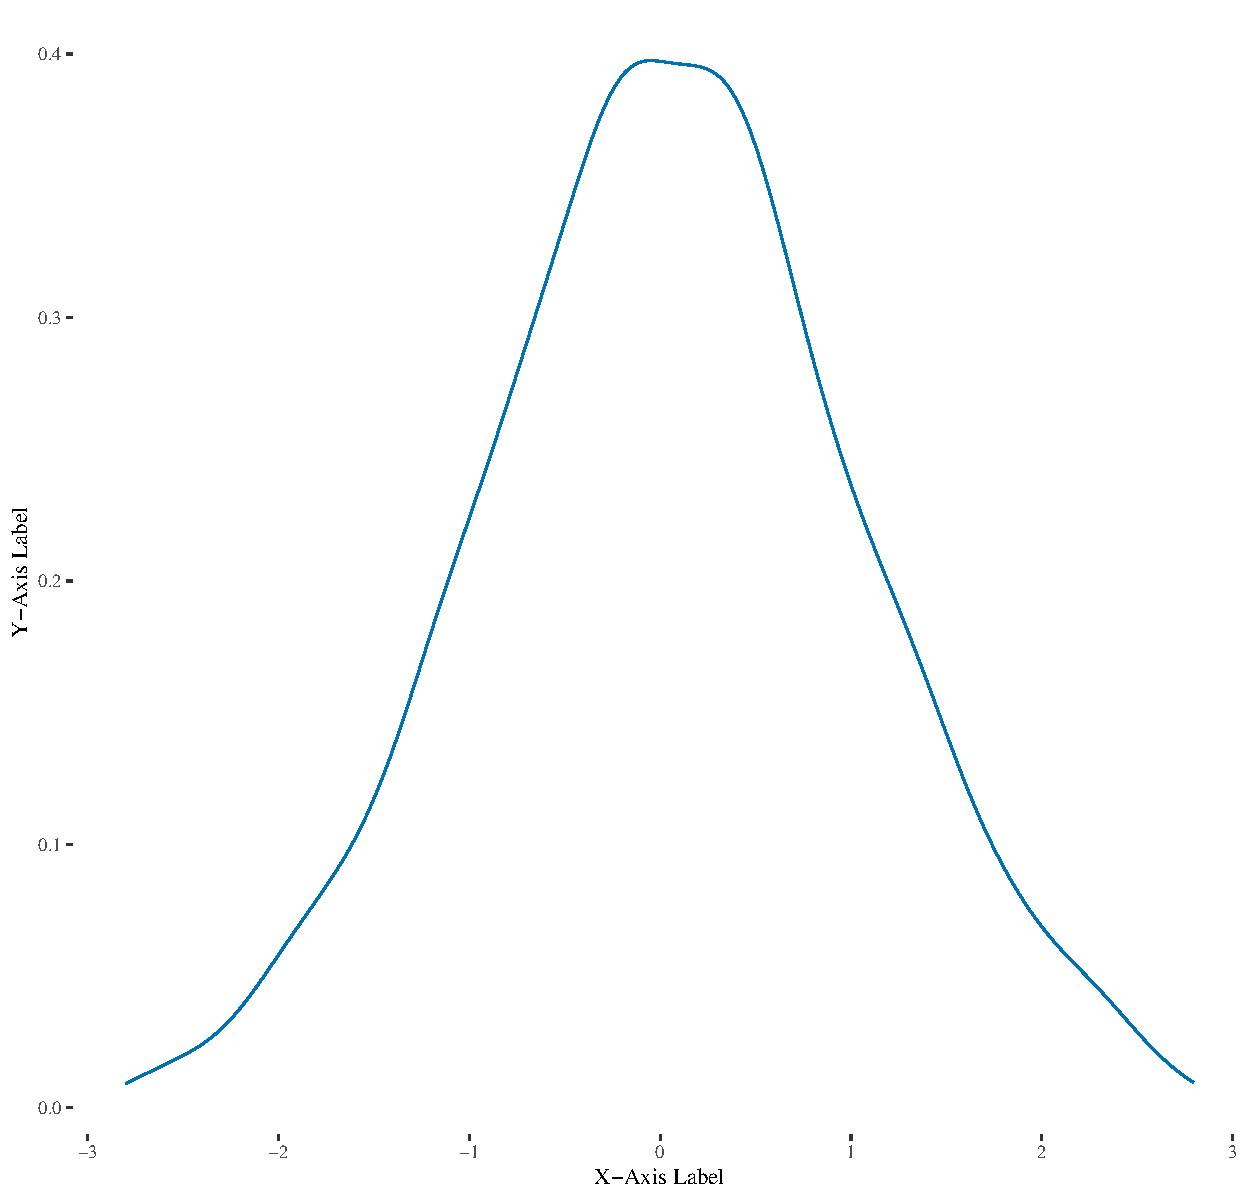
\includegraphics{figure_badlabels.pdf}
%    }
%  }
%}
%\only<2>{
%  \makebox[\linewidth][c]{
%    \resizebox{\linewidth}{!}{
%      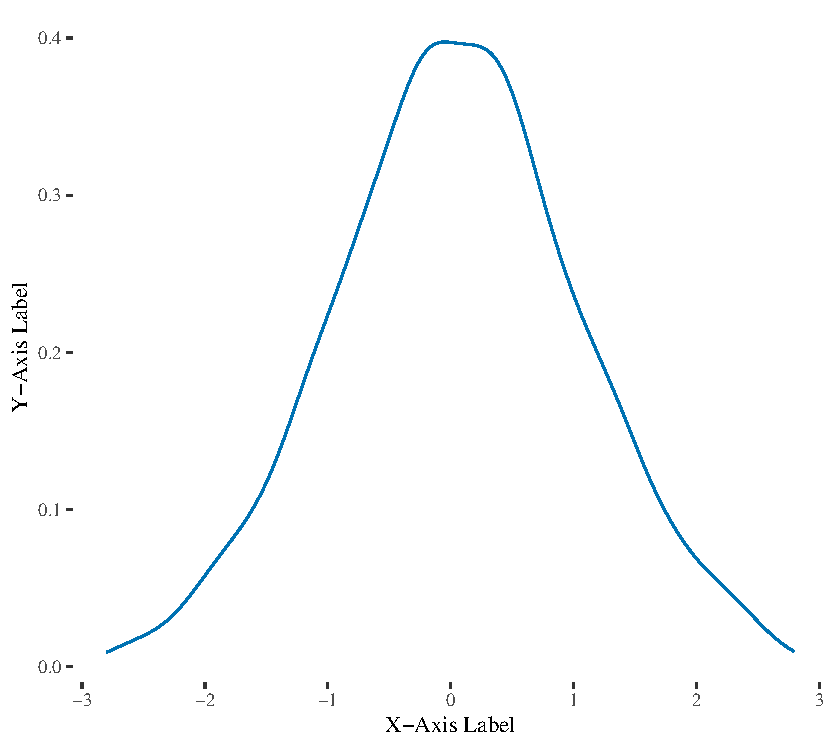
\includegraphics{figure_goodlabels.pdf}
%    }
%  }
%}
%\only<3>{
%  \makebox[\linewidth][c]{
%    \resizebox{\linewidth}{!}{
%      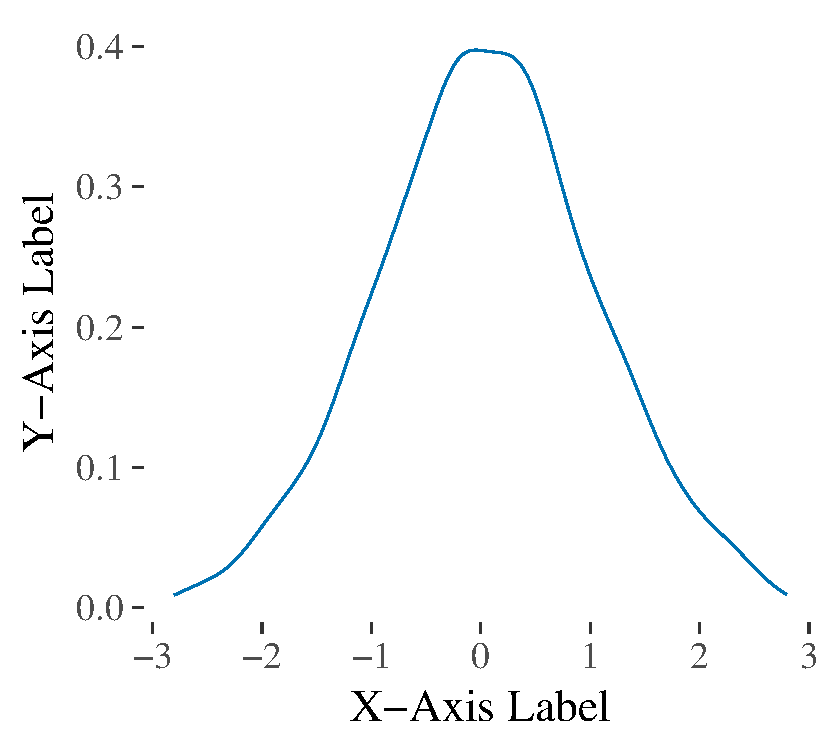
\includegraphics{figure_bestlabels.pdf}
%    }
%  }
%}
%\end{column}%
%\hfill%
%\begin{column}{.4\textwidth}
%  \begin{wideitemize}
%  \item[]<1-> This graph is unreadable! 
%  \item[$\rightarrow$]<1-> Need to change the font size
%  \item[]<2-> Now it looks a little better
%  \item[]<3-> \textcolor{red}{Much} better 
%  \item[]<3-> Things on your computer look too big but audience will thank you
%  \end{wideitemize}
%\end{column}%
%\end{columns}
%\end{frame}


%\begin{frame}[fragile]{Change your fonts!}
%  \begin{wideitemize}
%  \item[-] Changing fonts is easy and productive
%  \item[-] This slide deck uses Lato -- you can experiment!
%  \item[-] Here's some comparison to alternatives:\\
%    \begin{itemize}
%    \item[]    {Lato: the \textit{quick} \textbf{brown} fox jumps over the $\alpha$- dog}\\
%    \item[]     {\fontfamily{cmr}\selectfont  Arial (default): the \textit{quick} \textbf{brown} fox jumps over the $\alpha$- dog}\\
%    \item[]     {\fontfamily{pbk}\selectfont  Bookman: the \textit{quick} \textbf{brown} fox jumps over the $\alpha$- dog}\\
%    \item[]     {\fontfamily{phv}\selectfont  Helvetica: the \textit{quick} \textbf{brown} fox jumps over the $\alpha$- dog}\\
%    \end{itemize}
%  \end{wideitemize}
%  \bigskip
%  To change your font globally, you'll need to find the right package:
%  \begin{verbatim}
%   \usepackage[default]{lato}
%   \end{verbatim}
%  Link for choices: \url{http://www.tug.dk/FontCatalogue/sansseriffonts.html}
%\end{frame}


%\section{Dummy Frames}
%\begin{transitionframe}
%  \begin{center}
%    \Huge \textcolor{blue}{Dummy Frames}
%  \end{center}
%\end{transitionframe}
%
%
%\begin{frame}{Here's a list of frames that are similar to powerpoint frames}
%  \begin{wideitemize}
%    \item Just copy and paste the source code
%  \end{wideitemize}
%\end{frame}
%
%
%\begin{frame}{Two Column Frame}
%\begin{columns}[T] % align columns
%\begin{column}{.58\textwidth}
%\color{red}\rule{\linewidth}{4pt}
%Column 1
%\end{column}%
%\hfill%
%\begin{column}{.38\textwidth}
%\color{blue}\rule{\linewidth}{4pt}
%Column 2
%\end{column}%
%\end{columns}
%\end{frame}
%
%\begin{frame}
%  \vspace{-8pt}
%\begin{columns}[T] % align columns
%\begin{column}{.58\textwidth}
%\begin{minipage}[t][\textheight][t]
%  {\dimexpr\textwidth}
%  \vspace{8pt}
%  \hspace{4pt} \textcolor{red}{Two Column w/ Face}
%  \vspace{8pt}
%  
%Information goes here
%    \end{minipage}
%\end{column}%
%\hfill%
%\begin{column}{.42\textwidth}
% \colorbox{orange!20}{\begin{minipage}[t][1.2\textheight][t]
%      {\dimexpr\textwidth}
%      Face goes here
%    \end{minipage}}
%\end{column}%
%\end{columns}
%\end{frame}
%
%\begin{videoframe}{This Looks Good}
%  Using the Environ package
%\end{videoframe}
%
%\begin{frame}{Table Frame}
%\setbeamercovered{invisible}
%\makebox[\linewidth][c]{
%\begin{tabular}{l}
%\toprule
%Temp Table\\
%\bottomrule
%\end{tabular}
%}
%\end{frame}
%
%\begin{frame}{Figure Frame}
%\begin{center}
%\resizebox{0.5\textwidth}{!}{
%  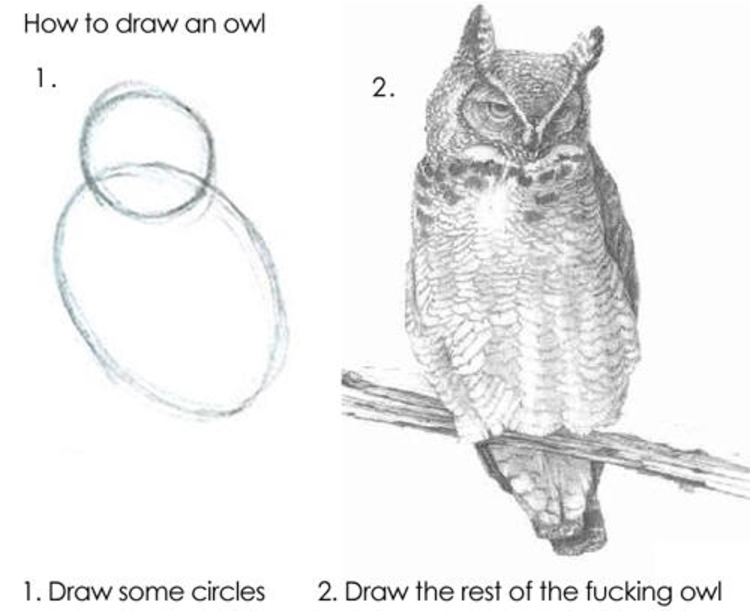
\includegraphics{how-to-draw-an-owl.pdf}
%}
%\end{center}
%\end{frame}
%
%\begin{frame}{Figure with Commentary Frame}
%\begin{columns}[T] % align columns
%\begin{column}{.58\textwidth}
%\resizebox{\textwidth}{!}{
%  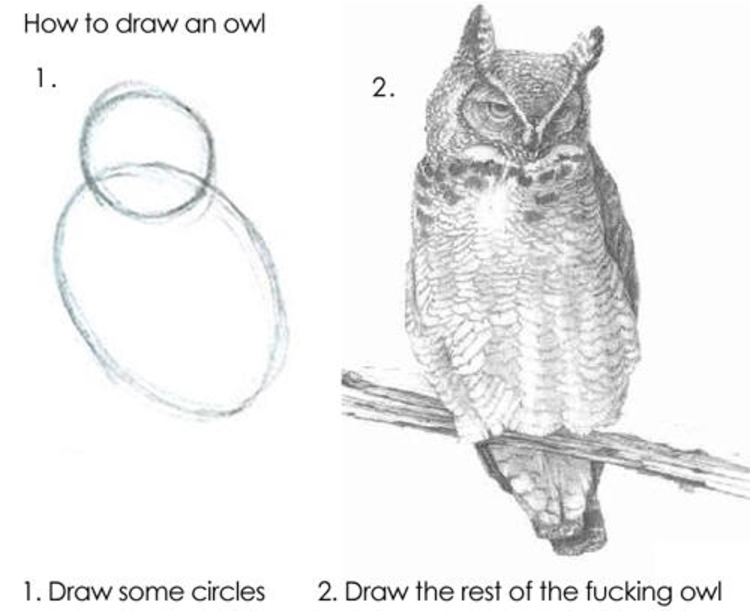
\includegraphics{how-to-draw-an-owl.pdf}
%}
%\end{column}%
%\hfill%
%\begin{column}{.38\textwidth}
%  \begin{wideitemize}
%  \item Everyone gives these tips on nice presentations
%  \item But maybe we'd put less on the slides
%  \item If the audience stopped interrupting
%  \end{wideitemize}
%\end{column}%
%\end{columns}
%\end{frame}


%\section{Misc and options to change}
%\begin{transitionframe}
%  \begin{center}
%    \Huge \textcolor{blue}{Miscellaneous + Options}
%  \end{center}
%\end{transitionframe}
%
%\begin{frame}{Make TikZ figures to help highlight your research design}
%  \begin{wideitemize}
%    \item Previously used tikz commands to highlight things in figures and tables
%    \item You can make much cooler figures with this
%    \item Here's an example for showing diff-in-diff timing:
%  \end{wideitemize}
%\begin{center}
%\begin{tikzpicture}[snake=zigzag, line before snake = 5mm, line after snake = 5mm, line width=1mm]
%    % draw horizontal line   
%    \draw (0,0) -- (1,0);
%    \draw[snake] (1,0) -- (3,0);
%    \draw (3,0) -- (4,0);
%    \draw[blue] (4,0) -- (8,0);
%    \draw[->] (8,0) -- (9,0);
%
%
%    \draw (0,.95) -- (1,.95);
%    \draw[snake] (1,.95) -- (3,.95);
%    \draw (3,.95) -- (4,.95);
%    \draw[red] (4,.95) -- (8,.95);
%    \draw[->] (8,.95) -- (9,.95);
%
%    % draw vertical lines
%    \foreach \x in {8}
%      \draw (\x cm,.205) -- (\x cm,-.205);
%    \foreach \x in {4}
%      \draw (\x cm,{.95+(.205)}) -- (\x cm,{.95-(.205)});
%    \foreach \x in {0}
%      \draw (\x cm,{.95+(.205)}) -- (\x cm,{0-(.205)});
%
%    % draw nodes
%    \draw (0,0) node[below=.105] {}  node[left=.105] {\textcolor{blue}{Control}};
%    \draw (0,0.95) node[below=.105] {} node[above=.105] {} node[left=.105] {\textcolor{red}{Treatment}};
%    \draw (4,.95) node[below=.105] {} node[above=.105] {} node[below=.105] {Policy Treatment};
%    \draw (8,0) node[below=.105] {} node[above=.105] {} node[below=.105] {End Policy};
%  \end{tikzpicture}
%\end{center}
%\end{frame}
%
%\begin{frame}{Consider making your math prettier}
%  \begin{wideitemize}
%    \item Don't overdo it when putting up equations\\(either regressions or theorems)
%    \item Try adding color and text to highlight the relevant formula
%    \item Consider (Imbens and Angrist 1994): 
%      \begin{equation*}
%        \alpha_{g}^{IV} = \left. \underbrace{Cov(Y, g(\textcolor{blue}{Z}))}_{\text{\textcolor{red}{Reduced Form}}} \middle/ \underbrace{Cov(D, g(\textcolor{blue}{Z}))}_{\text{\textcolor{green}{First Stage}}} \right.
%      \end{equation*}
%  \end{wideitemize}
%\end{frame}


% From here: https://tex.stackexchange.com/questions/114219/add-notes-to-latex-beamer
% To give a presentation with the Skim reader (http://skim-app.sourceforge.net) on OSX so
% that you see the notes on your laptop and the slides on the projector, do the following:
% 
% 1. Generate just the presentation (hide notes) and save to slides.pdf
% 2. Generate onlt the notes (show only nodes) and save to notes.pdf
% 3. With Skim open both slides.pdf and notes.pdf
% 4. Click on slides.pdf to bring it to front.
% 5. In Skim, under "View -> Presentation Option -> Synhcronized Noted Document"
%    select notes.pdf.
% 6. Now as you move around in slides.pdf the notes.pdf file will follow you.
% 7. Arrange windows so that notes.pdf is in full screen mode on your laptop
%    and slides.pdf is in presentation mode on the projector.
\note[itemize]{
\item Make sure not to forget notes!
\item I should use these more
\item put your text here!
}



\section{Appendix}
\begin{transitionframe}
  \begin{center}
    \Huge \textcolor{blue}{Appendix!}
  \end{center}
\end{transitionframe}

%\appendix

%\begin{frame}[label=appendix_start]{Almost done!}
%  \begin{wideitemize}
%  \item See, now we're in backup slide land
%  \item This is made useful by having links throughtout the talk
%  \item Here's a button, which is how I make links \hyperlink{appendix_end}{\beamergotobutton{Next slide}}
%  \end{wideitemize}
%\end{frame}
%
%\begin{frame}[label=appendix_end]{Use it to intimidate audiences!}
%  \begin{wideitemize}
%    \item[] Now you can make it clear you've done a shitload of work
%      \begin{itemize}
%      \item[]  without having to show everything! \hyperlink{appendix_start}{\beamergotobutton{Back}}
%      \end{itemize}
%    \item[] You label a frame with the \texttt{[label=name]} option, and then point a link to it
%    \item[] You can make an object a link using the \texttt{\textbackslash hyperlink\{label\}\{object\}} command
%  \end{wideitemize}
%\end{frame}


% Uncomment slide for bibliography
%\begin{frame}
%	\printbibliography
%\end{frame}


\end{document}
